\documentclass[12pt]{article}

%----------------- Packages ------------------
\usepackage[utf8]{inputenc}
\usepackage[T1]{fontenc}
\usepackage{amsmath, amssymb}
\usepackage{geometry}
\usepackage{xcolor}
\usepackage{titlesec}
\usepackage{fancyhdr}
\usepackage[breakable]{tcolorbox}
\usepackage{graphicx}
\usepackage{tikz}
\usepackage{float}
\usetikzlibrary{arrows.meta, decorations.markings}

%----------------- Page Setup -----------------
\geometry{a4paper, margin=2.5cm}
\pagestyle{fancy}
\fancyhf{}
\rhead{Normal Exam — \textbf{21-22}}
\lhead{Electricity I}
\cfoot{\thepage}

%----------------- Title Styling --------------
\titleformat{\section}{\normalfont\Large\bfseries}{Exercise \thesection:}{1em}{}
\titleformat{\subsection}{\normalfont\bfseries}{Answer:}{1em}{}

%----------------- Custom Boxes ----------------
\tcbuselibrary{listingsutf8}
\newtcolorbox{answerbox}{
  colback=gray!10,
  colframe=black,
  fonttitle=\bfseries,
  title=Answer Area,
  breakable,
  before skip=10pt,
  after skip=10pt
}

%----------------- Document Start --------------
\begin{document}

%----------------- Exam Info -------------------
\begin{center}
  \Large\textbf{Ibn Tofail University} \\[1em]
  \large\textit{Electricity I — Normal Exam} \\[0.5em]
  \large\textit{Year: 21-22} \\[2em]
\end{center}

\vspace{0.5cm}

%----------------- EXERCISE 1 ------------------
\section{}
Consider two point charges at rest $q$ and $-q$ placed respectively at points A and B on an $Ox$ axis (Figure 1).

\begin{figure}[H]
    \centering
    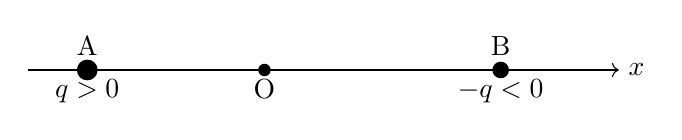
\begin{tikzpicture}[scale=1.5]
        % Draw the axis
        \draw[->] (-2,0) -- (3,0) node[right] {$x$};
        
        % Place points
        \fill[black] (-1.5,0) circle (2.5pt) node[below] {$q>0$};
        \node at (-1.5,0.2) {A};
        
        \fill[black] (0,0) circle (1.5pt) node[below] {O};
        
        \fill[black] (2,0) circle (2pt) node[below] {$-q<0$};
        \node at (2,0.2) {B};
    \end{tikzpicture} 
    \caption{}
\end{figure}



\begin{enumerate}
\item Give the vector expression of the electrostatic force $\vec{F}_{q/-q}$ created at B.
\item Give the vector expression of the electrostatic field $\vec{E}$ created at B.
\item Give the expression of the electrostatic potential $V$ created at B.
\end{enumerate}

\newpage

\begin{answerbox}
    \begin{enumerate}
        \item \textbf{Vector expression of the electrostatic force $ \vec{F}_{q \to -q} $ created at $ B $:}
    
        Using Coulomb's law:
        $$
        \vec{F}_{q \to -q} = \frac{1}{4\pi\varepsilon_0} \cdot \frac{q(-q)}{|\vec{r}_B - \vec{r}_A|^2} \cdot \frac{\vec{r}_B - \vec{r}_A}{|\vec{r}_B - \vec{r}_A|}
        $$
    
        Compute the vector $ \vec{r}_B - \vec{r}_A = d\vec{i} - (-d\vec{i}) = 2d\vec{i} $, so:
        $$
        \vec{F}_{q \to -q} = \frac{1}{4\pi\varepsilon_0} \cdot \frac{-q^2}{(2d)^2} \cdot \vec{i}
        = -\frac{q^2}{16\pi\varepsilon_0 d^2} \vec{i}
        $$
    
        Final expression:
        $$
        \boxed{\vec{F}_{q \to -q} = -\frac{q^2}{16\pi\varepsilon_0 d^2} \vec{i}}
        $$
    
        \item \textbf{Vector expression of the electrostatic field $ \vec{E} $ created at $ B $:}
    
        Electric field due to charge $ q $ at $ A $:
        $$
        \vec{E} = \frac{1}{4\pi\varepsilon_0} \cdot \frac{q}{|\vec{r}_B - \vec{r}_A|^2} \cdot \frac{\vec{r}_B - \vec{r}_A}{|\vec{r}_B - \vec{r}_A|}
        = \frac{1}{4\pi\varepsilon_0} \cdot \frac{q}{(2d)^2} \cdot \vec{i}
        = \frac{q}{16\pi\varepsilon_0 d^2} \vec{i}
        $$
    
        Final expression:
        $$
        \boxed{\vec{E} = \frac{q}{16\pi\varepsilon_0 d^2} \vec{i}}
        $$
    
        \item \textbf{Expression of the electrostatic potential $ V $ created at $ B $:}
    
        Electrostatic potential due to charge $ q $ at distance $ 2d $:
        $$
        V = \frac{1}{4\pi\varepsilon_0} \cdot \frac{q}{2d}
        = \frac{q}{8\pi\varepsilon_0 d}
        $$
    
        Final expression:
        $$
        \boxed{V = \frac{q}{8\pi\varepsilon_0 d}}
        $$
    \end{enumerate}
\end{answerbox}

\newpage

%----------------- EXERCISE 2 ------------------
\section{}
Consider two point charges at rest $q$ and $-q$ placed respectively at points A and B (Figure 2).
Given $OA = OB = a$.

\begin{figure}[H]
    \centering
\begin{tikzpicture}[scale=1.5]
    % Draw the axes
    \draw[->] (-3,0) -- (3,0) node[right] {$x$};
    \draw[->] (0,-1.5) -- (0,2) node[above] {$y$};
    
    % Place points
    \fill[black] (-1,1) circle (2pt) node[above left] {A};
    \node[left] at (-1,1) {$q$};
    
    \fill[black] (1,1) circle (2pt) node[above right] {B};
    \node[right] at (1,1) {$-q$};
    
    \fill[black] (0,0) circle (1.5pt) node[below left] {O};
    
    % Draw vectors
    \draw[->] (0,0) -- (0.7,0) node[below right] {$\vec{i}$};
    \draw[->] (0,0) -- (0,0.7) node[right] {$\vec{j}$};
    
    % Draw lines from O to A and O to B
    \draw[thin] (0,0) -- (-1,1);
    \draw[thin] (0,0) -- (1,1);
    \draw[thin] (-1,1) -- (1,1);
\end{tikzpicture}
\caption{}
\end{figure}

\begin{enumerate}
\item Give the vector expression of the electrostatic field $\vec{E} = E_x\vec{i} + E_y\vec{j}$ created at O.
\item Give the expression of the electrostatic potential $V$ created at O.
\end{enumerate}

\newpage

\begin{answerbox}
    \begin{enumerate}
        \item \textbf{Vector expression of the electrostatic field $ \vec{E} = E_x \vec{i} + E_y \vec{j} $ created at point $ O $:}
    
        Given:
        - Charge $ q $ is located at point $ A $, with coordinates $ (-a, 0) $
        - Charge $ -q $ is located at point $ B $, with coordinates $ (a, 0) $
        - Point $ O $ is the origin $ (0, 0) $
    
        The electric field at $ O $ is the vector sum of the fields due to both charges.
    
        
            
    - Electric field due to charge $ q $ at $ A $:
            $$
            \vec{E}_A = \frac{1}{4\pi\varepsilon_0} \cdot \frac{q}{a^2} \cdot \vec{i}
            $$
            (since it points toward the right)
    
            
    - Electric field due to charge $ -q $ at $ B $:
            $$
            \vec{E}_B = \frac{1}{4\pi\varepsilon_0} \cdot \frac{-q}{a^2} \cdot (-\vec{i}) = \frac{1}{4\pi\varepsilon_0} \cdot \frac{q}{a^2} \cdot \vec{i}
            $$
            (also pointing toward the right)
        
    
        Total electric field at $ O $:
        $$
        \vec{E} = \vec{E}_A + \vec{E}_B = \frac{1}{4\pi\varepsilon_0} \cdot \frac{q}{a^2} \vec{i} + \frac{1}{4\pi\varepsilon_0} \cdot \frac{q}{a^2} \vec{i} = \frac{1}{2\pi\varepsilon_0} \cdot \frac{q}{a^2} \vec{i}
        $$
    
        Final expression:
        $$
        \boxed{\vec{E} = \frac{q}{2\pi\varepsilon_0 a^2} \vec{i}}
        $$
    
        \item \textbf{Expression of the electrostatic potential $ V $ created at point $ O $:}
    
        Electrostatic potential is a scalar quantity. So we simply add the potentials from both charges:
    
        $$
        V = \frac{1}{4\pi\varepsilon_0} \left( \frac{q}{a} + \frac{-q}{a} \right) = \frac{1}{4\pi\varepsilon_0} \cdot 0 = 0
        $$
    
        Final expression:
        $$
        \boxed{V = 0}
        $$
    \end{enumerate}
\end{answerbox}

\newpage

%----------------- EXERCISE 3 ------------------
\section{}
A distribution of positive charges with linear density $\lambda$ is uniformly distributed along an infinitely long wire. Give the expression of the electrostatic field $\vec{E}$ created by this wire using Gauss's theorem.

\newpage

\begin{answerbox}
    \textbf{Expression of the electrostatic field $ \vec{E} $ created by an infinitely long wire with linear charge density $ \lambda $:}
    
    We are given a uniformly charged, infinitely long wire with linear charge density $ \lambda > 0 $. To find the electrostatic field $ \vec{E} $ at a distance $ r $ from the wire, we use \textbf{Gauss's theorem}.
   
    \begin{enumerate}
    \item \textbf{Choose a Gaussian surface}  
    Use a cylindrical surface of radius $ r $ and length $ L $, coaxial with the wire.
    
    \item \textbf{Apply Gauss’s Law}
    $$
    \Phi_E = \oint \vec{E} \cdot d\vec{S} = \frac{Q_{\text{enc}}}{\varepsilon_0}
    $$
    
    Since the electric field is radial and uniform in magnitude on the curved surface:
    $$
    E \cdot 2\pi r L = \frac{\lambda L}{\varepsilon_0}
    $$
    
    \item\textbf{Solve for $ E $:}
    $$
    E = \frac{\lambda}{2\pi\varepsilon_0 r}
    $$
    
    The direction of the field is radial. So the vector expression is:
    $$
    \vec{E} = \frac{\lambda}{2\pi\varepsilon_0 r} \vec{e}_r
    $$
    
    Final expression:
    $$
    \boxed{\vec{E} = \frac{\lambda}{2\pi\varepsilon_0 r} \vec{e}_r}
    $$
    \end{enumerate}
\end{answerbox}

\newpage

%----------------- EXERCISE 4 ------------------
\section{}
Consider a cylindrical capacitor consisting of two coaxial cylindrical plates of infinite length, with radii $R_1$ and $R_2$, separated by vacuum ($R_2 > R_1$) (Figure 3). Let $\sigma$ be the charge per unit area of the inner cylinder.
\begin{figure}[H]
\centering
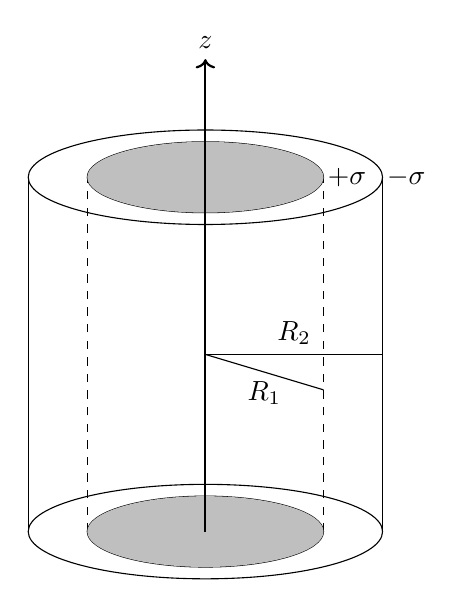
\begin{tikzpicture}[scale=1.5]

    % Draw the outer cylinder (dashed lines)
    \draw (-1.5,0) -- (-1.5,3);
    \draw(1.5,0) -- (1.5,3);
    
    % Squashed circular shapes for the top and bottom of the outer cylinder
    \draw (0,0) ellipse (1.5 and 0.4);
    \draw (0,3) ellipse (1.5 and 0.4);
    
    % Draw the inner cylinder (solid lines)
    \draw[dashed] (-1,0) -- (-1,3);
    \draw[dashed] (1,0) -- (1,3);
    
    % Squashed circular shapes for the top and bottom of the inner cylinder
    \draw (0,0) ellipse (1 and 0.3);
    \draw (0,3) ellipse (1 and 0.3);
    
    % Shade the regions R1 and R2
    \fill[gray!50] (0,0) ellipse (1 and 0.3);
    \fill[gray!50] (0,3) ellipse (1 and 0.3);
    
    % Label the radii R1 and R2
    \draw[] (0,1.5) -- (1,1.2) node[midway, below] {$R_1$};
    \draw[] (0,1.5) -- (1.5,1.5) node[midway, above] {$R_2$};
    
    % Draw the z-axis
    \draw[thick, ->] (0,0) -- (0,4) node[above] {$z$};
    
    % Add labels for sigma
    \node at (1.7,3) {$-\sigma$};
    \node at (1.2,3) {$+\sigma$};
    
    \end{tikzpicture}
\caption{}
\end{figure}

\begin{enumerate}
\item Give the expression for the capacitance $C$ of this cylindrical capacitor, knowing that, according to Gauss's theorem, the electrostatic field $\vec{E}$ between the two plates is written as:
$$
\vec{E} = \frac{\sigma}{\varepsilon_0} \frac{R_1}{r} \vec{e_r}
$$
\item Give the expression for the capacitance $C$ of this cylindrical capacitor if $e = R_2 - R_1 \ll R_1$.
\end{enumerate}

\newpage

\begin{answerbox}
    \begin{enumerate}
        \item \textbf{Expression for the capacitance $ C $ of the cylindrical capacitor:}
    
        Given:
        - Two coaxial cylindrical plates with radii $ R_1 $ and $ R_2 $, with $ R_2 > R_1 $
        - The electric field between the plates is given by:
        $$
        \vec{E} = \frac{\sigma R_1}{\varepsilon_0 r} \vec{e}_r
        $$
    
        To find the capacitance $ C $, we first compute the potential difference $ V $ between the two cylinders:
    
        $$
        V = \int_{R_1}^{R_2} \vec{E} \cdot d\vec{r} = \int_{R_1}^{R_2} \frac{\sigma R_1}{\varepsilon_0 r} dr
        = \frac{\sigma R_1}{\varepsilon_0} \ln\left( \frac{R_2}{R_1} \right)
        $$
    
        The charge per unit length on the inner cylinder is $ Q = \sigma \cdot 2\pi R_1 $
    
        Then the capacitance per unit length is:
        $$
        C = \frac{Q}{V} = \frac{\sigma 2\pi R_1}{\frac{\sigma R_1}{\varepsilon_0} \ln\left( \frac{R_2}{R_1} \right)} = \frac{2\pi\varepsilon_0}{\ln\left( \frac{R_2}{R_1} \right)}
        $$
    
        Final expression for the capacitance per unit length:
        $$
        \boxed{C = \frac{2\pi\varepsilon_0}{\ln\left( \frac{R_2}{R_1} \right)}}
        $$
    
        \item \textbf{Expression for the capacitance $ C $ when $ e = R_2 - R_1 \ll R_1 $:}
    
        In this case, the separation $ e $ is very small compared to $ R_1 $. So we can approximate:
        $$
        \ln\left( \frac{R_2}{R_1} \right) = \ln\left( 1 + \frac{e}{R_1} \right) \approx \frac{e}{R_1} \quad \text{(for small } \frac{e}{R_1})
        $$
    
        Substituting into the previous result:
        $$
        C \approx \frac{2\pi\varepsilon_0 R_1}{e}
        $$
    
        Alternatively, since the geometry resembles a parallel-plate capacitor when $ e \ll R_1 $, the result also makes sense as analogous to:
        $$
        C_{\text{parallel plate}} = \frac{\varepsilon_0 A}{e}
        $$
        where $ A = 2\pi R_1 L $ is the area for a cylinder of length $ L $.
    
        Final approximated expression:
        $$
        \boxed{C \approx \frac{2\pi\varepsilon_0 R_1}{e}}
        $$
    \end{enumerate}
\end{answerbox}

%----------------- END ------------------
\end{document}